\documentclass[lettersize,journal]{IEEEtran}
\usepackage{amsmath,amsfonts}
\usepackage{algorithmic}
\usepackage{array}
\usepackage[caption=false,font=normalsize,labelfont=sf,textfont=sf]{subfig}
\usepackage{textcomp}
\usepackage{stfloats}
\usepackage{url}
\usepackage{verbatim}
\usepackage{graphicx}
\hyphenation{op-tical net-works semi-conduc-tor IEEE-Xplore}
\def\BibTeX{{\rm B\kern-.05em{\sc i\kern-.025em b}\kern-.08em
    T\kern-.1667em\lower.7ex\hbox{E}\kern-.125emX}}
\usepackage{balance}
\begin{document}
\title{CPTR380 RISC-V RV32I FPGA Implementation}
\author{Jaron Brown & Ethan Jansen
\thanks{Manuscript created March, 2024.}}

\markboth{Journal of \LaTeX\ Class Files,~Vol.~18, No.~9, September~2020}%
{How to Use the IEEEtran \LaTeX \ Templates}

\maketitle

\begin{abstract}
TBD
\end{abstract}

\begin{IEEEkeywords}
ISA, RISC, RISC-V, RV32I FPGA, VHDL.
\end{IEEEkeywords}


\section{Introduction}
\IEEEPARstart{S}{ince} designing a custom ALU-based CPU last quarter in the Intro to Digital Design class, both of the authors developed an interest in implementing a more commonly supported instruction set architecture (ISA). When presented with the opportunity to pursue a project related to computer architecture in their Computer Architecture class, both authors jumped at the opportunity to implement another CPU design. They initially considered implementing the MIPS ISA but, after conducting more research, decided on implementing one of the RISC-V standard ISAs, RV32I. This decision was made based on the abundant documentation for the RISC-V ISAs, RV32I's relative simplicity, and the high commercial interest in these ISA specifications.
One of the dominant reasons many companies are developing RISC-V implementations is it open-source nature. The dominant ISAs (x86, ARM, MIPS, etc.) all have steep licensing fees. The RISC-V ISAs, in comparison, are completely free. Additionally, the closed-source nature of the dominant ISAs limits the freedom those designing implementation of these ISAs. Having a completely open-source ISA just makes sense--it lowers the barrier to entry for designing hardware to implement standard ISAs and allows for more innovation in the realm of CPU design.  

\section{A Brief Introduction to RISC-V}
\noindent The original design of RISC-V was begun in 2010 at the University of California, Berkeley. It was designed not only as an academic learning aid but also a set of ISAs that could have commercial viability. As its name suggests, RISC-V is a RISC (Reduced Instruction Set Computer) architecture. This means, in comparision to CISC (Complex Instruction Set Computer) ISAs, RISC ISAs have simple instructions. This means more individual instructions will be required to complete a given task compared to CISC ISAs but also allows the hardware implementation to be much simpler than that for CISC ISAs. In fact, implementations of x86-64, the most widely adopted CISC ISA, breaks its CISC instructions into "microinstructions" which are easier to implement in hardware, similar to RISC ISAs.
There has been reference to RISC-V ISAs. The reason for the plural ISAs is RISC-V is actually a collection of ISAs, ranging from 32-bit to 128-bit standards and supporting various levels of complexity by way of extensions to the base ISAs. Some official extensions include the M extension which adds multiplication and division support, the A extension whic adds support for atomic instructions, and the F and D extensions which add support for single- and double-precision floating numbers, respectively. Developers are encouraged to design their own compatible extensions to customize the base RISC-V ISA to their specific application. 

\section{Project Goals}
\noindent In this project, version 2.1 of the RV32I ISA will be implemented in VHDL and tested on a Xilinx Artix 7 FPGA (Field-Programmable Gate Array). RV32I is the RISC-V base integer ISA and implements the core functionality of the RISC-V architecture family. Although RV32 supports pipelining, this projects implemetation will not implement this feature due to time constrains. I/O, multiplication and division, full support for C code compilation, and pipelining, are stretch goals of this project. The authors hope to continue this project beyond their class and continue to refine the design and add more features.
 
\section{Implementation Overview}
\noindent This project's implementation of non-pipelined RV32I consists of a few core components: instruction memory, data memory, a register block, an ALU (Arithmetic Logic Unit), a control module, and various other components related to sign-extension, incrementing the program counter, and routing signals. Unlike the author's previous CPU designs which used and accumulator, this implementation uses a register block with 32 32-bit wide registers. This is in keeping with the RV32I standard and allows for more flexibility when programming the CPU.

\section{Conclusion}


\begin{thebibliography}{1}

\bibitem{ams}
{\it{Mathematics into Type}}, American Mathematical Society. Online available: 

\bibitem{oxford}
T.W. Chaundy, P.R. Barrett and C. Batey, {\it{The Printing of Mathematics}}, Oxford University Press. London, 1954.

\bibitem{lacomp}{\it{The \LaTeX Companion}}, by F. Mittelbach and M. Goossens

\bibitem{mmt}{\it{More Math into LaTeX}}, by G. Gr\"atzer

\bibitem{amstyle}{\it{AMS-StyleGuide-online.pdf,}} published by the American Mathematical Society

\bibitem{Sira3}
H. Sira-Ramirez. ``On the sliding mode control of nonlinear systems,'' \textit{Systems \& Control Letters}, vol. 19, pp. 303--312, 1992.

\bibitem{Levant}
A. Levant. ``Exact differentiation of signals with unbounded higher derivatives,''  in \textit{Proceedings of the 45th IEEE Conference on Decision and Control}, San Diego, California, USA, pp. 5585--5590, 2006.

\bibitem{Cedric}
M. Fliess, C. Join, and H. Sira-Ramirez. ``Non-linear estimation is easy,'' \textit{International Journal of Modelling, Identification and Control}, vol. 4, no. 1, pp. 12--27, 2008.

\bibitem{Ortega}
R. Ortega, A. Astolfi, G. Bastin, and H. Rodriguez. ``Stabilization of food-chain systems using a port-controlled Hamiltonian description,'' in \textit{Proceedings of the American Control Conference}, Chicago, Illinois, USA, pp. 2245--2249, 2000.

\end{thebibliography}

\begin{IEEEbiographynophoto}{Jane Doe}
Biography text here without a photo.
\end{IEEEbiographynophoto}

\begin{IEEEbiography}[{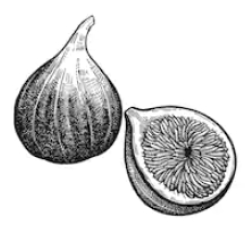
\includegraphics[width=1in,height=1.25in,clip,keepaspectratio]{fig1.png}}]{IEEE Publications Technology Team}
In this paragraph you can place your educational, professional background and research and other interests.\end{IEEEbiography}


\end{document}


